\documentclass [12pt] {oblivoir}

\usepackage{fapapersize}
\usefapapersize{210mm,297mm,20mm,*,20mm,22mm}

\setlength\parindent{0pt}

\usepackage{graphicx}
\usepackage{mathtools}
\usepackage{amsmath}
\usepackage{upgreek}

\begin{document}
양서류에 속하는 한 동물종에서 최근 새로 발견된 $S$세포는 거의 평면에 가까운 평평한 형태를 갖고 있다.
게다가 주변의 제약이 없을 경우 완전한 정사각형 모양을 가지며 계속하여 자라나 더 큰 정사각형의 형태가 된다고 한다.

실험실에서 당신은 배양지에 $S$세포를 가능한 큰 정사각형 모양으로 키우는 과제를 부여 받았다.
하지만 배양지에는 불순물이 함유되어 있으며 $S$세포는 불순물에 닿게 되면 즉시 성장을 멈추고 그때까지의 크기를 계속 유지하게 된다.
배양지의 크기는 무한히 크며, 따라서 평면 전체를 이룬다고 가정하자.
불순물은 이 평면에서 총 $N$ 개의 점들로 나타난다.
배양하기 전의 $S$세포는 변의 길이가 0 에 가까운 정사각형 형태이며 배양지에서 미리 주어진 $x$ 축 위의 선분 $L$ 위의 어떤 한 점에 정착시켜야 한다.
실험에서는 단 한 개의 $S$세포만을 정착하며, 시간이 지난 후에 이 $S$세포는 불순물에 닿을 때까지 자라 최초에 정착한 점을 중심으로 하는 정사각형 모양이 된다.
배양지를 나타내는 평면에 총 $N$ 개의 불순물의 위치가 좌표로 주어지고 선분 $L$

이 주어질 때, 당신이 키울 수 있는 $S$세포의 최대 크기는 얼마일까?
이때의 정사각형의 한 변의 길이를 출력하는 프로그램을 작성하시오.

단, 최초에 $S$세포를 정착시킬 때에는 모양이 축에 평행한 정사각형이 되도록 한다고 가정한다.
또한, 이렇게 정착한 $S$세포는 이후에도 늘 축에 평행한 정사각형을 이루며 자라나며 배양지에 완전히 밀착된 상태를 유지한다고 가정한다.

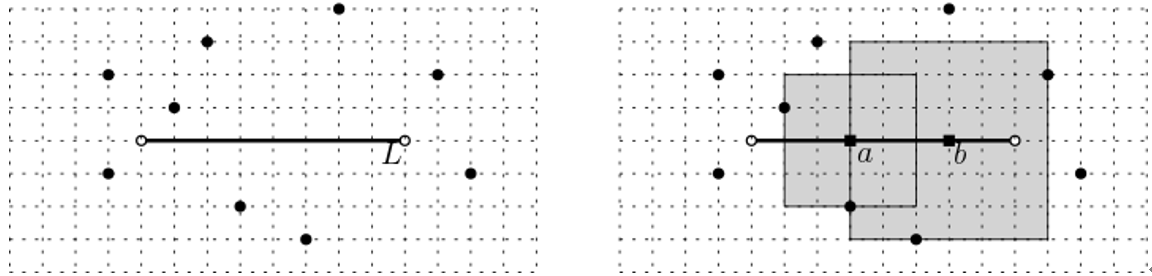
\includegraphics[scale=0.5]{n5.png}

예를 들어,  위 그림의 왼쪽과 같이 선분 $L$ 이 주어지고 배양지에 총 9개의 불순물 위치가 주어져 있다고 가정하자. (그림에서 점선으로 표시된 격자의 최소 길이는 1이다.)
이 때, 오른쪽 그림에서 보이는 바와 같이, 점 $a$ 에 $S$ 세포를 최초 정착했다면 변의 길이가 4인 정사각형 모양까지 자라나게 되는 반면, 점 $b$에 $S$ 세포를 최초 정착했다면 이 세포는 변의 길이가 6인 정사각형 모양까지 자라나게 된다.
이 경우는 6이 가능한 최대 크기가 되므로 당신의 프로그램은 6을 출력해야 한다.


- 제한시간: 전체 테스트 케이스는 40개 이하이며, 전체 수행 시간은 2초 이내. (Java 4초 이내)

제한 시간을 초과하면 제출한 소스코드의 프로그램이 즉시 종료되며,
그때까지 수행한 결과에서 테스트 케이스를 1개 그룹 이상 통과하였더라도 점수는 0점이 됩니다.
그러나, 제한 시간을 초과하더라도 테스트 케이스를 1개 그룹 이상 통과하였다면 '부분 점수(0 $<$ 점수 $<$ 만점)'를 받을 수 있으며,
이를 위해서는, C / C++ 에서 "printf 함수" 사용할 경우, 프로그램 시작부분에서 "setbuf(stdout, NULL);"를 한번만 사용하십시오.
C++에서는 "setbuf(stdout, NULL);"와 "printf 함수" 대신 "cout"를 사용하고, Java에서는 "System.out.printIn"을 사용하시면,
한 시간을 초과하더라도 '부분 점수'를 받을 수 있습니다.

※ 언어별 기본 제공 소스코드 내용 참고

만약, 제한 시간을 초과하지 않았는데도 '부분 점수'를 받았다면, 일부 테스트 케이스를 통과하지 못한 경우 입니다.

- 메모리 사용 제한 : heap, global, static 총계 256MB, stack 100MB

- 제출 제한 : 최대 10회 (제출 횟수를 반영하여 순위 결정 → 동점자의 경우 제출 횟수가 적은 사람에게 높은 순위 부여)

메모리 사용 제한

heap, global, static (총계) : 256MB

stack : 100MB

입력

입력 파일에는 여러 테스트 케이스가 포함될 수 있다.

파일의 첫째 줄에 테스트 케이스의 개수를 나타내는 자연수 $T$가 주어지고,

이후 차례로  T 개의 테스트 케이스가 주어진다. $(1 \le T \le 40)$

각 테스트 케이스의 첫 줄에는 두 개의 정수 $l, r(-1012 \le l < r \le 1012)$가 공백으로 구분되어 주어지며, $(l, 0)$ 과 $(r, 0)$는 각각 선분 L 의 왼쪽 및 오른쪽 끝점의 좌표가 된다.

두번째 줄에는 한 개의 정수 $N(1 \le N \le 100,000)$이 주어지는데, 이는 불순물의 개수를 나타낸다.

다음 N 개의 줄의 i 번째 줄에는 두 정수 $x_{i}, y_{i}(-1012 \le x_{i}, y_{i} \le 1012)$가 공백으로 구분되어 주어지며, 각 $(x_{i}, y_{i})$는 불순물의 좌표를 의미한다.

- 점수 : 최대 10회 제출하여 취득한 각각의 점수 중에서 최대 점수 (만점 200점)

모든 테스트 케이스를 맞추었을 때 만점을 받는다.

주어지는 테스트 케이스 데이터들의 그룹은 아래와 같으며, 각 그룹의 테스트 케이스를 모두 맞추었을 때 해당되는 부분 점수를 받을 수 있다.

   ㆍ 그룹 1 (22 점) : 이 그룹의 테스트 케이스에서는 $N \le 100$ 이고 각 불순물의 좌표 $(x_{i}, y_{i})$는 $-105 \le x_{i}, y_{i} \le 105$ 을 만족한다. 또한, $-105 \le l < r \le 105$ 을 만족한다.

   ㆍ 그룹 2 (76 점) : 이 그룹의 테스트 케이스에서는 $N \le 100$이다.

   ㆍ 그룹 3 (102 점) : 이 그룹의 테스트 케이스에서는 별도의 제한이 없다.

출력

각 테스트 케이스의 답을 순서대로 표준출력으로 출력하여야 하며,

각 테스트 케이스마다 첫 줄에는 “Case \#C”를 출력하여야 한다. 이때 $C$는 테스트 케이스의 번호이다.

그 다음 줄에, 당신이 키울 수 있는 최대 크기의 $S$세포에 대해 그때의 정사각형의 한 변의 길이를 정수 형태로 출력하시오.

입출력예

입력

2

0 5

2

3 3

2 -3

0 8

9

1 1

2 3

6 4

9 2

10 -1

-1 -1

-1 2

3 -2

5 -3

출력

Case \#1

6

Case \#2

6
\end{document}
